\documentclass{ximera}

%% Where to find images
\graphicspath{  %% When looking for images,
{./}            %% look first at your level,
{./basics/}     %% then in this folder,
}

% might be overwritten in printstyle, to get a proper back cover for this course
\providecommand{\backCover}{}

\title{Textbooks}
\author{Bart Snapp}

\begin{document}
\pdfOnly{\onecolumn\begin{multicols}{2}}
\begin{abstract}
  You can write textbooks in Ximera.
\end{abstract}
\maketitle
This section is about \textit{best practices} when writing an entire
textbook.
\begin{description}
  \item[Keep related content in the same folder] to help yourself and
    others find content. For example, it is helpful to keep exercises that
    complement a section of a textbook in the same folder as that section.
  \item[Give descriptive names] to help others and your future self find things.
    Abstract names like \verb!chapter1! and \verb!course! are too generic, and
    are
    at best unhelpful and at worst confusing when things are rearranged.
  \item[Pay attention to file paths] as every file with a documentclass must
    compile, which could mean that files need to find the \verb!preamble.tex! file.
\end{description}

% \begin{verbatim}
% %% where to look for inputs
% \makeatletter
% \def\input@path{
% {./}
% {./coverArt/}
% {./introduction/}
% }
% \makeatother
% \end{verbatim}
\pdfOnly{\end{multicols}}

\begin{center}
  \scalebox{.7}{
    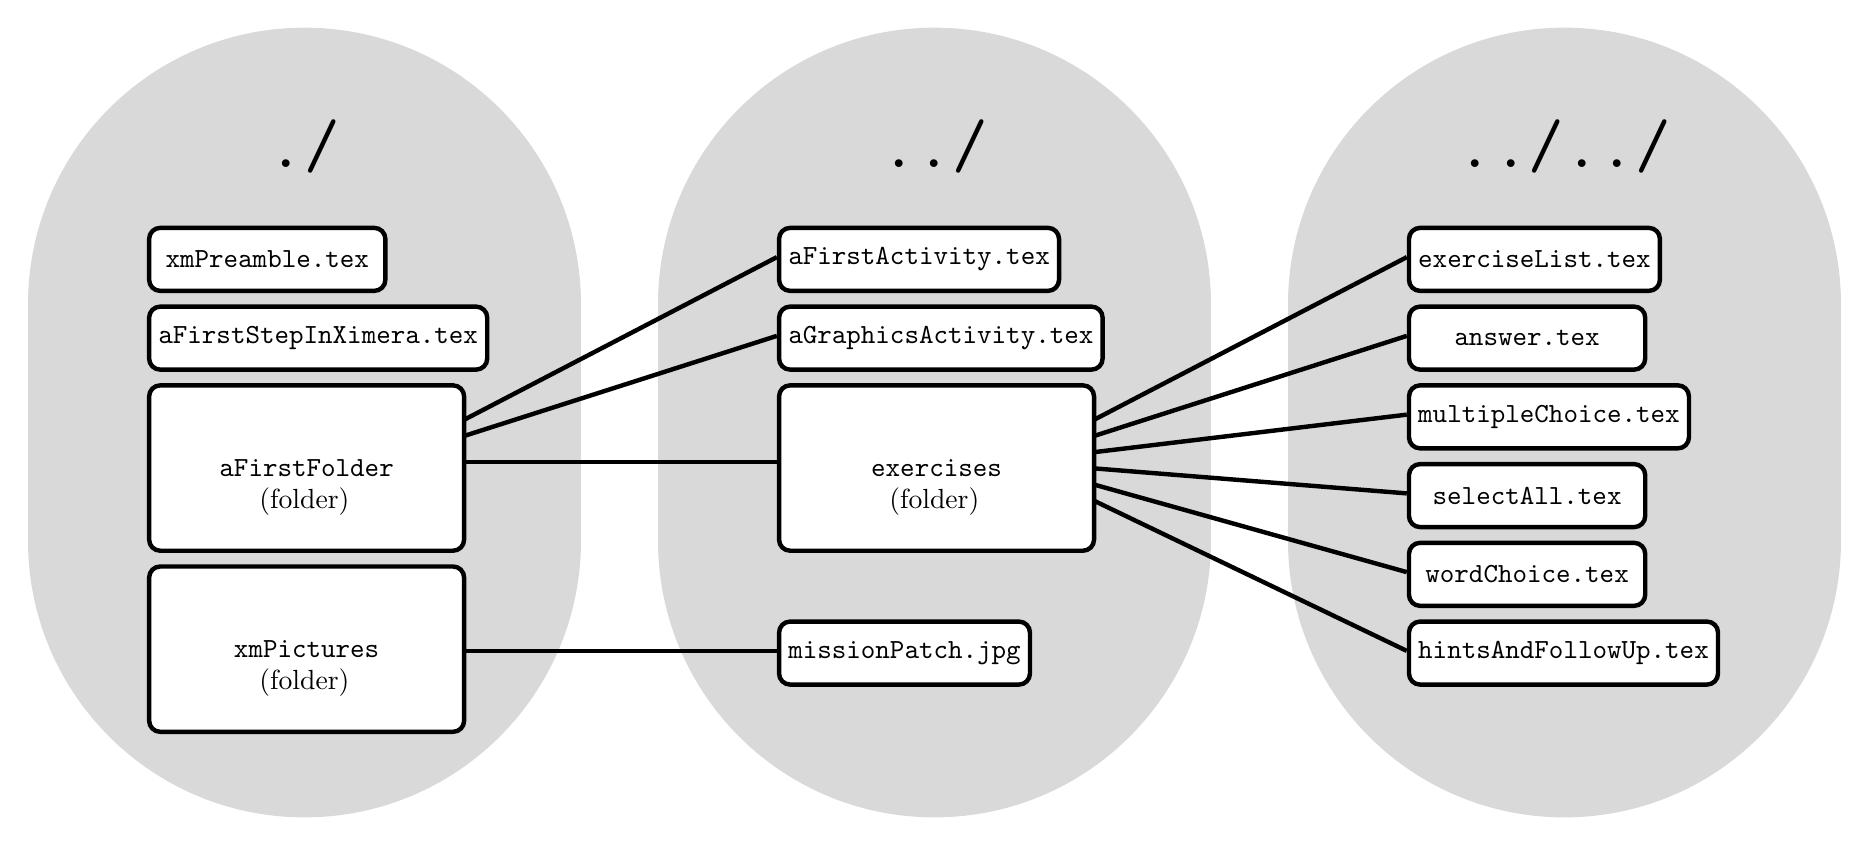
\begin{tikzpicture}
      % Define styles for nodes
      \tikzstyle{document} = [anchor=north west,draw, rounded corners,
      rectangle,
      minimum width=3cm,fill=white, minimum height=.8cm, ultra
      thick,font=\ttfamily]
      \tikzstyle{folder} = [anchor=north west,draw, rectangle, rounded corners,
      minimum width=4cm,fill=white, minimum height=2.1cm, ultra
      thick,font=\ttfamily]

      % Thick grey lines
      \draw[line width=200pt,white!85!black,line cap=round] (2,2) -- (2,-1);
      \draw[line width=200pt,white!85!black,line cap=round] (10,2) -- (10,-1);
      \draw[line width=200pt,white!85!black,line cap=round] (18,2) -- (18,-1);

      % Connections
      \draw[ultra thick] (3,0.0) -- (8,2.6);
      \draw[ultra thick] (3,0.0) -- (8,1.6);
      \draw[ultra thick] (3,0.0) -- (8,0);

      \draw[ultra thick] (3,-2.4) -- (8,-2.4);

      \draw[ultra thick] (11,0) -- (16,2.6);
      \draw[ultra thick] (11,0) -- (16,1.6);
      \draw[ultra thick] (11,0) -- (16,.6);
      \draw[ultra thick] (11,0) -- (16,-.4);
      \draw[ultra thick] (11,0) -- (16,-1.4);
      \draw[ultra thick] (11,0) -- (16,-2.4);


      % Symbols at top
      \node at (2,4) {\Huge \tt ./};
      \node at (10,4) {\Huge \tt ../};
      \node at (18,4) {\Huge \tt ../../};

      % Define the folders at top level
      \node[document] at (0,3) {xmPreamble.tex};
      \node[document] at (0,2) {aFirstStepInXimera.tex};
      \node[folder] at (0,1) {aFirstFolder};
      \node[] at (2,-.5) {(folder)};
      \node[folder] at (0,-1.3) {xmPictures};
      \node[] at (2,-2.8) {(folder)};

      % Define the documents in the basics folder
      \node[document] at (8,3) {aFirstActivity.tex};
      \node[document] at (8,2) {aGraphicsActivity.tex};
      \node[folder] at (8,1) {exercises};
      \node[] at (10,-.5) {(folder)};
      \node[document] at (8,-2) {missionPatch.jpg};

      % Define the documents in the exercises folder
      \node[document] at (16,3) {exerciseList.tex};
      \node[document] at (16,2) {answer.tex};
      \node[document] at (16,1) {multipleChoice.tex};
      \node[document] at (16,0) {selectAll.tex};
      \node[document] at (16,-1) {wordChoice.tex};
      \node[document] at (16,-2) {hintsAndFollowUp.tex};

    \end{tikzpicture}
  }
\end{center}
\pdfOnly{\twocolumn}


To help organize your book, you should use the documentclass option \verb!numbers! along with  \texttt{\textbackslash chapterstyle} and 
\texttt{\textbackslash sectionstyle}. Keep your sections short and sweet. Two things that authors commonly do are:
\begin{itemize}
  \item When you give a definition, ask a question after to check comprehension. 
  \item When you give an example, give an explanation with
        \texttt{\textbackslash answer} boxes to fill in.
\end{itemize}
\end{document}
